\documentclass{tufte-handout}

\title{Assignment-5: Cache Model, Address Translation and TLB}
  
  \author[]{Arnab Das, u1014840}
  
  %\date{28 March 2010} % without \date command, current date is supplied
  
  %\geometry{showframe} % display margins for debugging page layout
  
  % preamble.tex

\usepackage{graphicx} % allow embedded images
    \setkeys{Gin}{width=\linewidth,totalheight=\textheight,keepaspectratio}
    \graphicspath{{graphics/}} % set of paths to search for images
  \usepackage{tikz}
  \usetikzlibrary{shapes.geometric, arrows}
  \usepackage{amsmath}  % extended mathematics
  \usepackage{booktabs} % book-quality tables
  \usepackage{units}    % non-stacked fractions and better unit spacing
  \usepackage{multicol} % multiple column layout facilities
  \usepackage{lipsum}   % filler text
  \usepackage{fancyvrb} % extended verbatim environments
    \fvset{fontsize=\normalsize}% default font size for fancy-verbatim environments
  \usepackage{amsthm}
  \usepackage{thmtools}
  \usepackage{amssymb}
  %\usepackage[table]{xcolor}
  \usepackage{color}

  \newcommand*{\QEDA}{\hfill\ensuremath{\blacksquare}}%

  \newcommand{\stall}{\textcolor{red}{Stall}}
  %\newcommand{\cellstall}{\cellcolor{red}\textcolor{white}{\textbf{Stall}}}

  % Standardize command font styles and environments
  \newcommand{\doccmd}[1]{\texttt{\textbackslash#1}}% command name -- adds backslash automatically
  \newcommand{\docopt}[1]{\ensuremath{\langle}\textrm{\textit{#1}}\ensuremath{\rangle}}% optional command argument
  \newcommand{\docarg}[1]{\textrm{\textit{#1}}}% (required) command argument
  \newcommand{\docenv}[1]{\textsf{#1}}% environment name
  \newcommand{\docpkg}[1]{\texttt{#1}}% package name
  \newcommand{\doccls}[1]{\texttt{#1}}% document class name
  \newcommand{\docclsopt}[1]{\texttt{#1}}% document class option name
  \newenvironment{docspec}{\begin{quote}\noindent}{\end{quote}}% command specification environment
  \declaretheorem[thmbox=S]{theorem}
  \declaretheoremstyle[
spaceabove=6pt, spacebelow=6pt,
headfont=\normalfont\bfseries,
notefont=\mdseries, notebraces={(}{)},
bodyfont=\normalfont,
postheadspace=1em,
qed=\qedsymbol
]{mystyle}
\declaretheorem[style=mystyle,numbered=no]{Proof}
\declaretheorem[thmbox=S]{example}
\declaretheorem[thmbox=S]{Definition}

  
  \begin{document}
  
  \maketitle% this prints the handout title, author, and date
  

 \setcounter{secnumdepth}{1}

\newpage

	\section{$\textbf{Virtually Indexed Cache}$}
		The virtual address space is decomposed primarily into two fields, namely the virtual page number and the offset field. The virtual page number is used as the key to lookup the TLB or in case of TLB miss the page table, to find the corresponding page number of the physical address. Generally the virtual page and the physical page are of the same size, in which case thje offset field of the virtual address space directly maps to the "index"+"byte" field of the physical address, hence the offset can be used directly to index inside the cache, while in parallel the virtual address translation proceeds which is called the virtually indexed physically tagged.
		\paragraph{} However, several complications arise if the page offset does not equals the (index+byte) field of the physical address. This results in the physical page size and the virtual page size being different and hence we cannot directly use the virtual address offset to index into the cache. Two cases may arise due to this. Firstly, the virtual page size is larger than the the physical page(frame) size, or secondly the virtual page size is less than the physical page(frame) size. Both the situations are discussed below.
		\paragraph{$\textbf{Case-1: Page offset less than the (index+byte)}$}
			In this situation more than one virtual addresses(VA) can map to the same physical address. This situation has two side effects, one relating to stale data and the other relating to memory utilization.
			\begin{itemize}
				\item If more than one VA maps to the same PA, then it is possible to have multiple copies of the same physical address in TLB and stale data in the cache. For example, suppose adress $PQR$ and $XYZ$ both map to the same physial address $ABC$. First one process generates a request for $PQR$, its a cache miss and data is fetched from main memory, and the cache and TLB are both updated. Next if a request is generated for $XYZ$, it will again be a miss since it's entry does not exists in the TLB, although it's corresponding physical address $ABC$ is already in the cache. This results in a new copy of $ABC$ being accessed from memory, and TLB and cache being updated with a redundant copy. Now suppose a write happens to $PQR$, it will update its corresponding copy of the physical memory in the cache, but $XYZ$ will still be pointing to the stale value of $ABC$. This is referred to as the $synonym$ or $\textbf{aliasing}$ problem.
				\item Also, since the page offset is less than the (index+byte) field, only the offset field will be used to access into the physical frames in the cache. This results in underutilization of cache, since the full block is not being indexed. For example, suppose the page offset is 10 bits, where 8 bits are for indexing and 2 bits are for byte access. If the physical page, that is, the cache set size is larger say 12 bits, with 10 index bits and 2 offset bits, only the lower order 8 bits of index field would be valid corresponding to the 8 index bits of the offset field of the virtual page.
			\end{itemize}
			$\textbf{Solution:}$ To solve the $aliasing$ problem, we need to ensure primarily that multiple VA's do not map to same PA, or even if they do, there is a coherency protocol to be maintanied to updated the PA when any of the corresponding VA's existing in the tlb gets accessed. Thus we can do the following
			\begin{itemize}
				\item If same data exists in multiple cache lines, do a search in the cache to update all copies of the data, whenever any of the corresponding VA is accessed.
				\item To avoid the synonym problem, set the cache size to be equal to the page size times the associativity. This ensures that the page size is equal to the cache set size. If not, then multiple copies of the same data can exists in different cache sets.
				\item Requiring that all VA's that map to same PA, are made to access the same cache set, using cache coloring, where the corresponding physical address bits are artificially made to be equal to be the same as the virtual address bits used for indexing.
				\item Using page splintering, where the guest uses large page sizes but the hypervisor in the OS can limit those page sizes to match the frame size granularity.
			\end{itemize}

		\paragraph{$\textbf{Case-2: Page offset larger than the (index + byte)}$}
			In this situation the virtual page size is larger than the physical frame size. In case of a single process system this is not an issue, since  the virtual page number uniquely idenitfies a physical page, but the indexing into the cache needs to happen using the page offset of the physical address which is equal to the lower index bits of the virtual address. For example if the page offset is 12 bits with 10 bits index and 2 bits byte access while the physical address has 8 bits index and 2 bits offset, the indexing into the cache is required to happen with 8 bits index and 2 bits byte offset. The 2 extra index bits in the offset will be redundant, since the virtual page number uniquely identifies the physical page. However, in case of a multiprocessing/multitasking system $\textbf{this may not hold}$. Suppose , in this example we have a 22 bit address, which means the virtual tag is 10 bits while the physical tag is 12 bits. Thus, virtual address from different processes can have the same virtual tag of 10 bits, mapping to different PA's, hence the tag does not uniquely identifies the cache data. This is called the $homonym$ problem leading to incorrect data access.
			\paragraph{Solutions} To prevent the homonym problem,
			\begin{itemize}
				\item Additionally tag the virtual addresses with the corresponding address space identifier to identify that they belong to different physical addresses even though the virtual tags match.
				\item Or, one can use the physical tags to correctly index into the cache after translation from the tlb. This introduces extra cycles in the critical path since the translation first happens and then based on the translated address, the cache is indexed.
				\item Since this issue is mainly pertinent to multiprocess systems, whenever there is a context switch, flush the cache to ensure avoiding incorrect data access.
				\item Single address space operating system(SASOS) : In SASOS design, there is a single large address space use by all the processes, and maps this large space onto physical memory. A single address space ensures virtual addresses from different preocesses do not have the same virtual tag, thus avoiding the conflict.
			\end{itemize}


\section{$\textbf{Cache and Memory Model using CACTI)}$}
	CACTI-6.5 was used to analyze the impact of the given L1 and L2 parameters. For a 4GB adress space, number of address bits is 32. The tag bits were computed from the given cache size as follows
	\subsection{$\textbf{L1-cache configuration}$}
		\begin{eqnarray*}	
			\mbox{Cache Size } &=& 32 KB = 2^{15} B \\
			\mbox{Block Size} &=& 32 B = 2^5 B \\
			\mbox{\# of blocks} &=&  \dfrac{Cache\ Size}{Block\ Size} = 2^{10} \\
			\mbox{\# index bits} &=& 10 \\ 
			\mbox{\# byte offset bits} &=& 5 \\
			\mbox{\# Tag bits} &=& 32 - 15 = \mathbf{17} \\ 
		\end{eqnarray*}

	\subsection{$\textbf{L2-cache configuration}$}
		\begin{eqnarray*}	
			\mbox{Cache Size } &=& 1 MB = 2^{20} B \\
			\mbox{Cache line} &=& 64 B = 2^6 B \\
			\mbox{Associativity} &=& 4 \\
			\mbox{\# of cache sets} &=&  \dfrac{Cache\ Size}{Cache\ set\ size} = 2^{20-(6+2)} = 2^{12} \\
			\mbox{\# index bits} &=& 12 \\ 
			\mbox{\# byte offset bits} &=& 6 \\
			\mbox{\# Tag bits} &=& 32 - (12+6) = \mathbf{14} \\ 
		\end{eqnarray*}

		Cacti was run with the above tag bits and the configuration specified in figure:~\ref{fig:initConfig}.
		\begin{figure}[h!]
		\label{fig:initConfig}
		\centering
		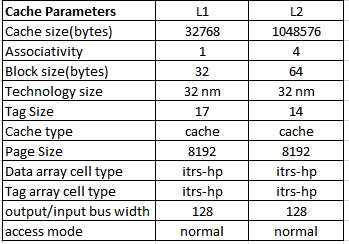
\includegraphics[width = 4in, height = 4in]{initConfig}
		\caption{L1 and L2 Configuration }
		\end{figure}

		\begin{itemize}
			\item The input-output bus-width was chosen to be $128$ bits such that an entire block of L1-cache(16 B) can be moved in a burst. 
			\item The Data and tag array cell type is chosen for high power as per the ITRS(International Technology Roadmap for Semiconductors) standard.
			\item For comparison between L1 and L2  cache , the access mode is set to normal. Later we compare between normal and fast access mode for L2 cache
		\end{itemize}

		Figure:~\ref{fig:L1L2Compare} shows the table for comparing the access time, energy, leakage power and area of L1 and L2 caches.
		\begin{figure}[h!]
		\label{fig:L1L2Compare}
		\centering
		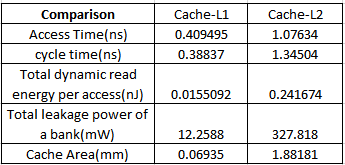
\includegraphics[width = 4in, height = 4in]{L1L2Compare}
		\caption{L1 and L2 Comparison }
		\end{figure}

		Below are the observations made from the comparative study
		\begin{itemize}
			\item We expect the access time of L1-cache to be much faster than the L2-cache. This is because the L1 cache is much smaller in size and hence the data access takes shorter time for L1 than L2. 
			\item Since the L2-cache is a much larger structure with 4 cache lines, the data path to access an  L-2 cache element requires more work since it is required to travel a larger circuitry. This is reflected by the dynamic read energy per access.
			\item Also, the leakage power consumption from L2 will be higher since it is built of sram that has high power consumption to hold the charge level in the component transistors. Although L1 is built of sram as well, its smaller structure makes its leakage power consumption much lower than L2.
			\item The cache area of the larger cache with multiple cache lines is expected to be higher, hence L2 has larger cache area than L1.
		\end{itemize}


	\subsection{$\textbf{L2-cache associativity}$}
	Here we perform a comparative study for L2-caches with different values of $n$ for its n-way associativity. The associativity is varied between $1-16$ in powers of 2, and the tag size is adjusted accordingly as shown
	\begin{eqnarray*}
		\mbox{1-way} &=& 12\ Tag\ bits \\
		\mbox{2-way} &=& 13\ Tag\ bits \\
		\mbox{4-way} &=& 14\ Tag\ bits \\
		\mbox{8-way} &=& 15\ Tag\ bits \\
		\mbox{16-way} &=& 16\ Tag\ bits \\
	\end{eqnarray*}

	We have run cacti for L2 in both Fast and normal access modes. Figure:~\ref{fig:compL2TabFast} and Figure:~\ref{fig:compL2TabNormal} shows the comparative data for different values of $n$ for fast and normal access modes respectively.
		\begin{figure}[h!]
		\label{fig:compL2TabFast}
		\centering
		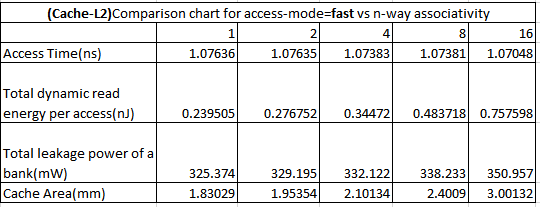
\includegraphics[width = 4in, height = 4in]{compL2TabFast}
		\caption{n-way comparison for fast access }
		\end{figure}

		
		\begin{figure}[h!]
		\label{fig:compL2TabNormal}
		\centering
		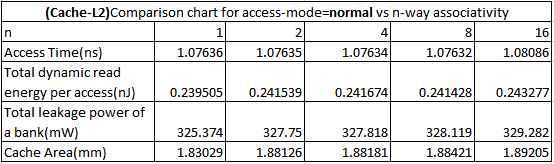
\includegraphics[width = 4in, height = 4in]{compL2TabNormal}
		\caption{n-way comparison for normal access }
		\end{figure}

		Figure: ~\ref{fig:accesstime}, Figure:~\ref{fig:dynamicenergy}, Figure:~\ref{fig:leakagepower} and Figure:~\ref{fig:cachearea} show the comparative graphs for access time, energy, leakage power and cache area respectively in nomral and fast mode access for varying associativity.

		
		\begin{figure}[h!]
		\label{fig:accesstime}
		\centering
		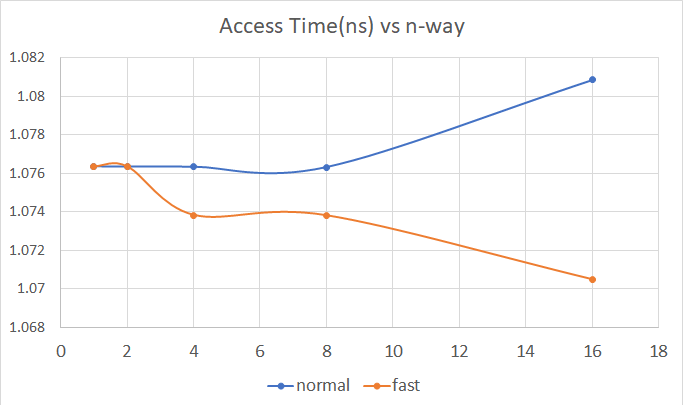
\includegraphics[width = 4in, height = 4in]{accesstime}
		\caption{n-way L2 access time }
		\end{figure}

		\begin{figure}[h!]
		\label{fig:dynamicenergy}
		\centering
		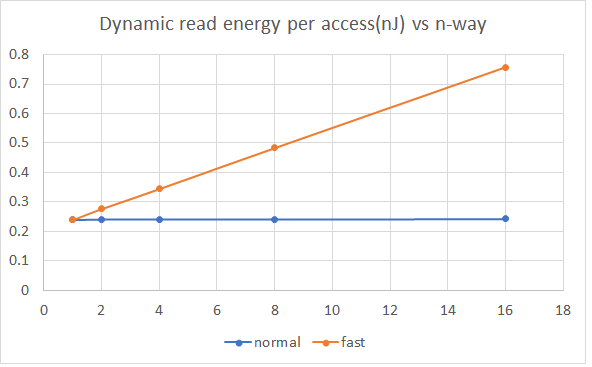
\includegraphics[width = 4in, height = 4in]{dynamicenergy}
		\caption{n-way L2 Dynamic energy per read access }
		\end{figure}

		\begin{figure}[h!]
		\label{fig:leakagepower}
		\centering
		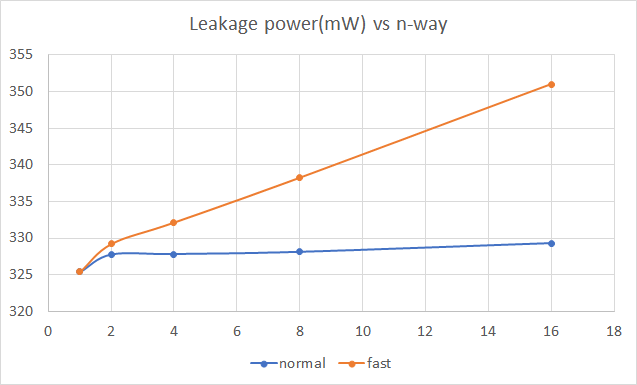
\includegraphics[width = 4in, height = 4in]{leakagepower}
		\caption{n-way L2 leakage power }
		\end{figure}

		\begin{figure}[h!]
		\label{fig:cachearea}
		\centering
		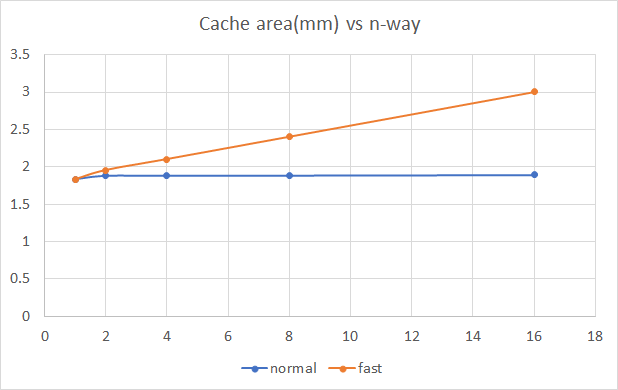
\includegraphics[width = 4in, height = 4in]{cachearea}
		\caption{n-way L2 cache area }
		\end{figure}

		The observations are listed below
		\begin{itemize}
			\item The access time tends to improve with increasing the associativity both in normal and fast mode, however in fast mode the drop in access time is much faster. Also, increasing associativity beyond 8 increases the access time in normal mode. In fast mode we see that drop in access time continues at n=16, but the drop rate reduces indicating it is reaching a saturation point beyond which increasing asociativity results in more overhead than improvement in access time.
			\item The fast access shows much larger swing in dynamic read energy with increasing cache lines, since with more parallelism, more hardware is active for a read in a given cycle .
			\item The leakage power also increses with increasing associativity, mainly due to more area of the hardware being active with multiple cache lines. The leakage power is also much higher when in fast access since introducing parallelism increases the volume of active circuitary.
			\item Increasing the number of cache lines incurs higher overhead in area to include the additional circuitry for the cache lines showing the incresing trend in area as we increase the associativity. In fast access mode, even more circuitary is deployed for enhacing parallel access to data hence significantly increasing the area overhead.
		\end{itemize}

		\section{$\textbf{References}$}
		\begin{itemize}
			\item \url{http://www.cse.unsw.edu.au/~cs9242/02/lectures/03-cache/node8.html}
			\item \url{https://www.cs.rutgers.edu/~abhib/binhpham-tr15.pdf}
			\item \url{http://www.cs.utah.edu/~naveen/cacti_report.pdf}
			\item \url{www.semiconductors.org/clientuploads/Research_Technology/ITRS/2005/1_Executive\%20Summary.pdf}
			\item \url{http://infocenter.arm.com/help/index.jsp?topic=/com.arm.doc.faqs/ka16862.html}
			\item \url{https://view.officeapps.live.com/op/view.aspx?src=http://www.cs.utah.edu/~rajeev/cacti6/micro07.ppt}
			\item \url{https://www.freebsd.org/doc/en_US.ISO8859-1/articles/vm-design/page-coloring-optimizations.html}
			\item \url{http://www.cs.rochester.edu/~sandhya/csc256/seminars/lingxiang_page_coloring.pdf}
		\end{itemize}






  \bibliography{cs6810}
  \bibliographystyle{plainnat}
  
  \end{document}
